% 建议使用 XeLaTeX 或 LuaLaTeX 编译(中文与公式支持更佳)
\documentclass[UTF8,zihao=-4]{ctexart}

\usepackage[a4paper,margin=2.5cm]{geometry}
\usepackage{amsmath, amssymb, amsthm}
\usepackage{bm}
\usepackage{hyperref}
\usepackage{graphicx}
\usepackage{caption}
\usepackage{listings}
\usepackage{xcolor}
\usepackage{float}
\usepackage{placeins}
\graphicspath{{figures/}}

\lstdefinestyle{code}{
  basicstyle=\ttfamily\small,
  numbers=left,
  numberstyle=\tiny,
  numbersep=8pt,
  keywordstyle=\color{blue},
  commentstyle=\color{teal!70!black},
  stringstyle=\color{orange!70!black},
  showstringspaces=false,
  breaklines=true,
  frame=single,
  framerule=0.3pt,
  rulecolor=\color{black!15}
}
\lstset{style=code}

\title{UMAP:原理、公式、应用与实战}
\author{}
\date{\today}

\begin{document}
\maketitle

\section{引言}
UMAP(Uniform Manifold Approximation and Projection)基于流形学习与拓扑数据分析,是一种常用的非线性降维算法。它在原空间构建加权邻接图,保留局部连通性,再优化低维嵌入以还原这些邻域关系,生成适合探索分析与聚类诊断的可视化布局。

\section{原理与公式}
\subsection{邻接图构建}
对每个样本 \(\mathbf{x}_i\),UMAP 选取 \(k\) 个最近邻,并使用平滑指数核计算边权:
\begin{equation}
\mu_{ij} = \exp\left(-\frac{\max(0, d(\mathbf{x}_i, \mathbf{x}_j) - \rho_i)}{\sigma_i}\right),
\end{equation}
其中 \(d\) 为距离度量,\(\rho_i\) 确保至少存在距离为零的邻居,\(\sigma_i\) 用于归一化局部连通性。将有向边对称化得到模糊拓扑表示:
\begin{equation}
\mathbf{W} = \mu + \mu^{\top} - \mu \odot \mu^{\top}.
\end{equation}

\subsection{低维优化}
UMAP 通过最小化高、低维模糊集合之间的交叉熵,学习低维嵌入 \(\mathbf{y}_i\)。嵌入空间的连接强度采用可微曲线:
\begin{equation}
\nu_{ij} = \frac{1}{1 + a\lVert \mathbf{y}_i - \mathbf{y}_j \rVert_2^{2b}},
\end{equation}
参数 \(a, b\) 根据距离分布拟合。损失函数为
\begin{equation}
C = \sum_{(i,j)} \left[ w_{ij} \log \frac{w_{ij}}{\nu_{ij}} + (1 - w_{ij}) \log \frac{1 - w_{ij}}{1 - \nu_{ij}} \right],
\end{equation}
采用随机梯度下降对采样边进行优化。

\subsection{超参数与实践要点}
关键参数包括邻居数 
_neighbors(控制局部与全局平衡)、min_dist(影响簇的松紧度)、距离度量以及初始化方式(spectral、
andom 或 PCA)。UMAP 通过近似最近邻与负采样处理大规模数据,但结果会随随机种子变化,建议多次运行取平均或挑选稳定解。

\section{应用与技巧}
\begin{itemize}
  \item \textbf{单细胞数据分析}:识别基因表达中的多样细胞类型与稀有群体。
  \item \textbf{文本与嵌入评估}:在语句或文档嵌入上观察语义簇是否清晰。
  \item \textbf{异常诊断}:结合时间或元数据信息,突出异常点或过渡态。
  \item \textbf{实用建议}:先做特征标准化,尝试多组 
_neighbors/min_dist 组合,对嵌入图做标签标注,并与 t-SNE、PCA 结果对照。
\end{itemize}

\section{Python 实战}
脚本 \texttt{gen\_t\_umap\_figures.py} 对合成数据标准化后,在不同邻居数下运行 UMAP,并计算衡量邻域保持度的 trustworthiness 指标,输出嵌入图与评分曲线。
\begin{lstlisting}[language=Python,caption={脚本 gen_t_umap_figures.py 片段}]
import umap
from sklearn.manifold import trustworthiness

neighbors_list = [10, 30, 50]
embeddings = {}
trust_scores = []
for n in neighbors_list:
    reducer = umap.UMAP(n_neighbors=n, min_dist=0.1, metric="euclidean",
                        init="spectral", random_state=42)
    embedding = reducer.fit_transform(points)
    embeddings[n] = embedding
    trust_scores.append(trustworthiness(points, embedding, n_neighbors=15))
\end{lstlisting}

\section{实验结果}
\begin{figure}[H]
  \centering
  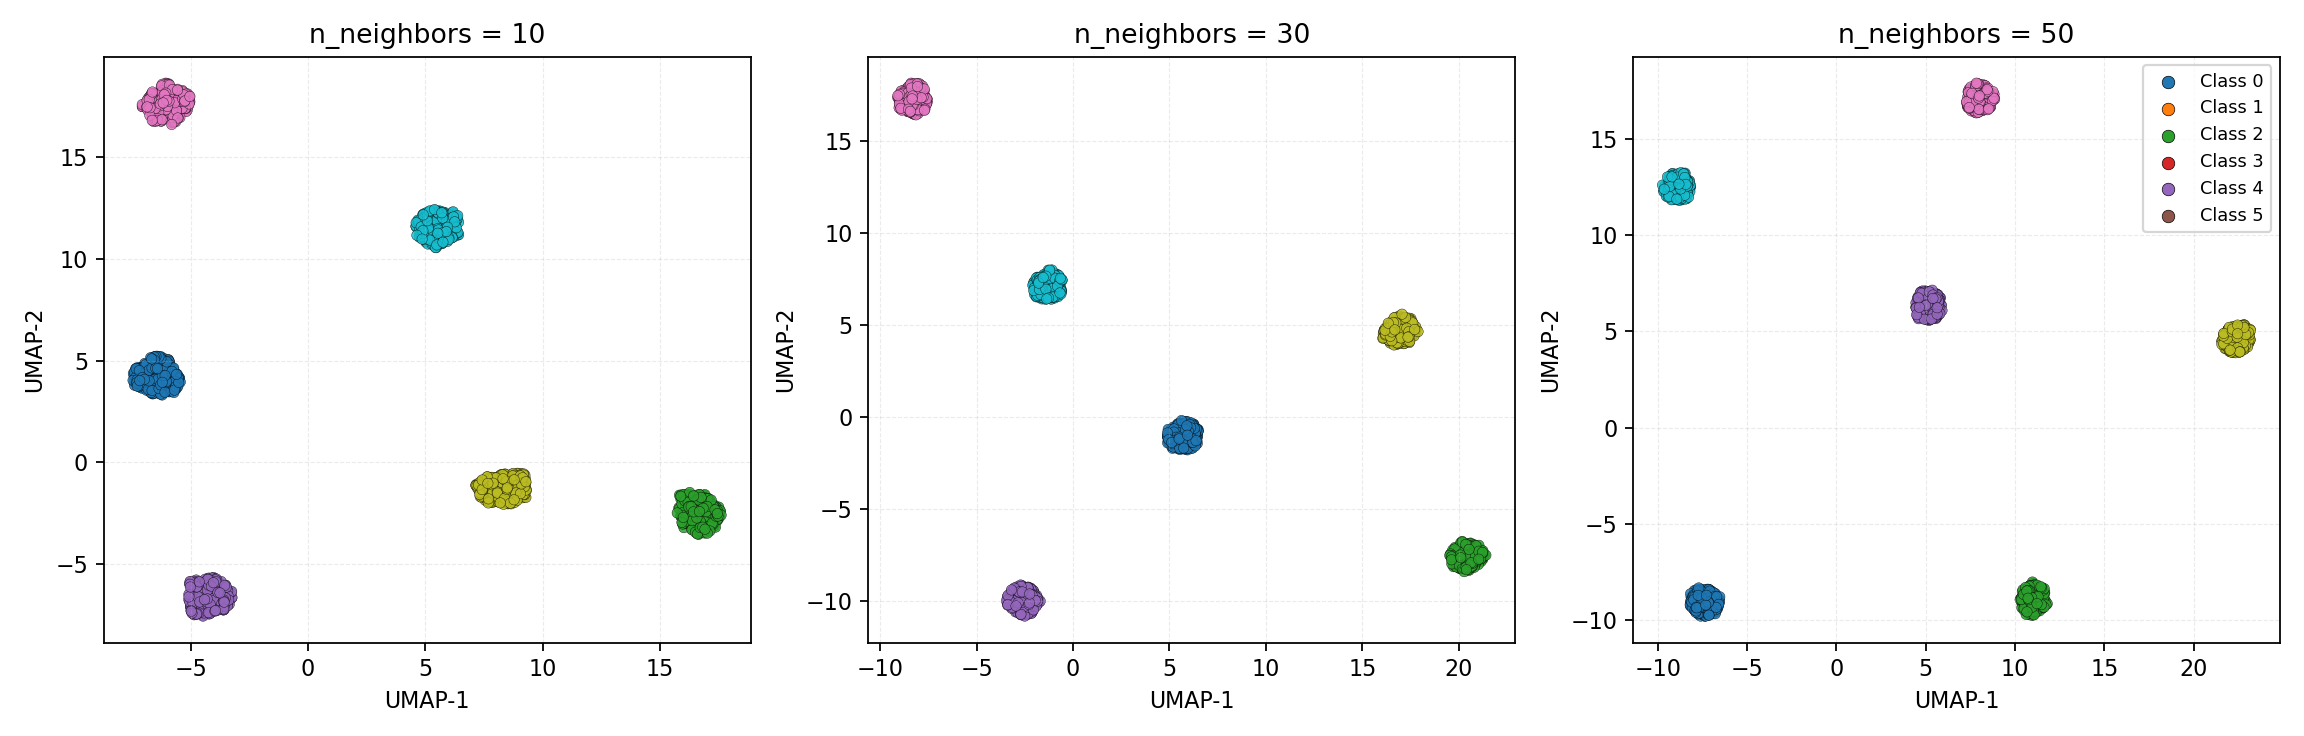
\includegraphics[width=0.82\linewidth]{umap_embeddings.png}
  \caption{不同邻居数下的 UMAP 嵌入,可根据类别着色}
  \label{fig:umap_embeddings_cn}
\end{figure}

\begin{figure}[H]
  \centering
  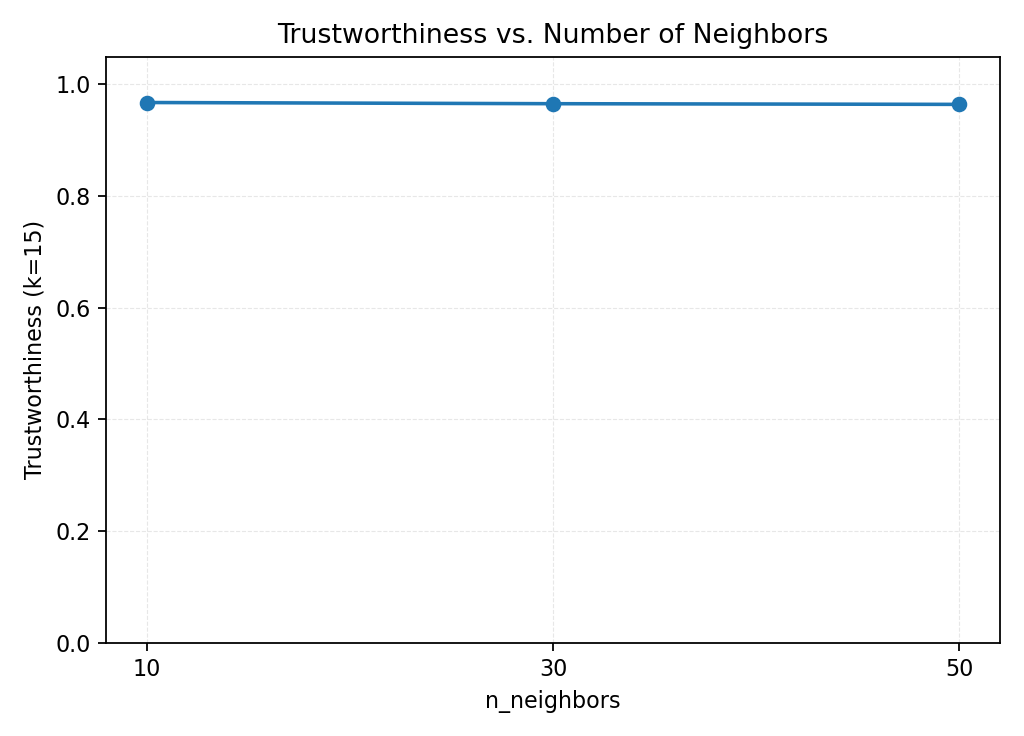
\includegraphics[width=0.8\linewidth]{umap_neighbor_curve.png}
  \caption{trustworthiness 指标随邻居数量变化的曲线}
  \label{fig:umap_neighbor_curve_cn}
\end{figure}

\FloatBarrier
\section{总结}
UMAP 通过模糊邻域建模与交叉熵优化兼顾局部细节与全局布局。合理调整邻居数、最小距离和距离度量,可在探索分析中获得稳定、易解读的嵌入图。示例展示了如何比较不同参数下的结果并利用 trustworthiness 曲线评估嵌入质量。

\end{document}